\chapter{Gregori Alexandrovitch Margulis --- Fields Medal 1978}\label{ch1978gregorialexandrovitchmargulis:gregori-alexandrovitch-margulis-fields-medal-1978}

\begin{center}\rule{0.5\linewidth}{0.5pt}\end{center}

\textbf{Prepared:} July 2026 \textbf{Subject:} Gregori Alexandrovitch
Margulis (b. February 24, 1946, Moscow, USSR) \textbf{Position:}
Professor, Yale University \textbf{Doctoral Advisor:} Yakov Sinai
(Moscow State University) \textbf{Fields Medal Citation:} ``For his
analysis of the structure of Lie groups, particularly his proof of the
superrigidity and arithmeticity conjectures.''

\begin{center}\rule{0.5\linewidth}{0.5pt}\end{center}

\section{Introduction}\label{ch1978gregorialexandrovitchmargulis:introduction}

Gregori Alexandrovitch Margulis is one of the most significant and
influential mathematicians of the late twentieth and early twenty-first
centuries. Awarded the Fields Medal in 1978, Margulis's work has
consistently reshaped the boundaries between seemingly disparate fields
of mathematics. By combining the techniques of ergodic theory, Lie
groups, algebraic geometry, number theory, and combinatorics, Margulis
solved several long-standing conjectures that had resisted the efforts
of generations of mathematicians. His research is characterized by an
notable ability to find hidden structures and bridges between
continuous symmetry and discrete arithmetic properties.

Throughout his career, Margulis has demonstrated a unique mathematical
style. Rather than confining himself to a single subdiscipline, he has
repeatedly solved deep problems in one area by introducing ideas and
techniques from another. For example, he solved the classical Oppenheim
Conjecture in number theory---which concerns the values of quadratic
forms at integer points---not through traditional number-theoretic or
analytic methods, but by translating it into a problem about the
dynamics of unipotent flows on homogeneous spaces. Similarly, he
constructed the first explicit families of expander graphs, a
fundamental object in computer science, by utilizing the representation
theory of Lie groups, specifically Kazhdan's Property (T).

\begin{figure}[htbp]
\centering
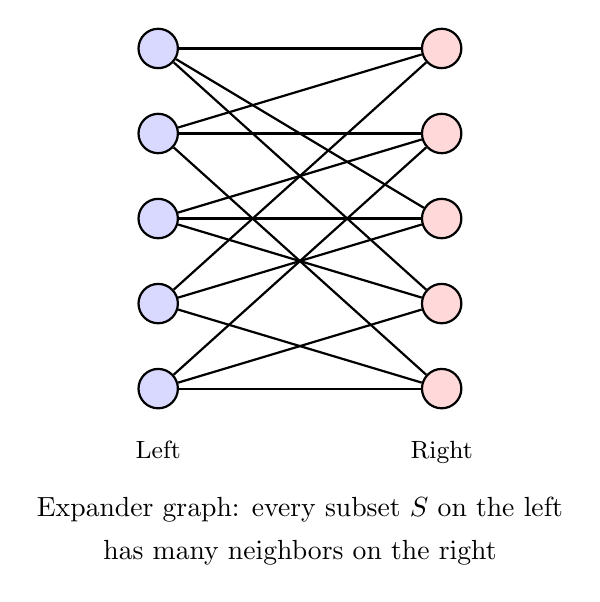
\begin{tikzpicture}[scale=0.9]
  % Expander graph: a bipartite graph with good expansion
  % Left vertices
  \foreach \i in {1,...,5} {
    \node[circle, draw, thick, fill=blue!15, minimum size=0.5cm] (L\i) at (0, \i*1.2) {};
  }
  % Right vertices
  \foreach \i in {1,...,5} {
    \node[circle, draw, thick, fill=red!15, minimum size=0.5cm] (R\i) at (4, \i*1.2) {};
  }
  
  % Edges (each left vertex connects to ~3 right vertices)
  \draw[thick] (L1) -- (R1); \draw[thick] (L1) -- (R2); \draw[thick] (L1) -- (R4);
  \draw[thick] (L2) -- (R1); \draw[thick] (L2) -- (R3); \draw[thick] (L2) -- (R5);
  \draw[thick] (L3) -- (R2); \draw[thick] (L3) -- (R3); \draw[thick] (L3) -- (R4);
  \draw[thick] (L4) -- (R1); \draw[thick] (L4) -- (R4); \draw[thick] (L4) -- (R5);
  \draw[thick] (L5) -- (R2); \draw[thick] (L5) -- (R3); \draw[thick] (L5) -- (R5);
  
  % Labels
  \node[below] at (0,0.6) {\small Left};
  \node[below] at (4,0.6) {\small Right};
  \node[below] at (2,-0.2) {Expander graph: every subset \(S\) on the left};
  \node[below] at (2,-0.8) {has many neighbors on the right};
\end{tikzpicture}
\caption{An expander graph: a sparse graph where every small subset of vertices has a disproportionately large set of neighbors. Margulis constructed the first explicit family using representation theory.}
\label{fig:expander-graph}
\end{figure}

This comprehensive report is structured to explore all facets of
Margulis's life, his mathematical creations, and their lasting legacy.
We survey his early life and education in the Soviet Union, the
mathematical foundations of Lie groups and lattices, his seminal proofs
of the superrigidity and arithmeticity conjectures, his contributions to
differential geometry, expander graphs, homogeneous dynamics, and the
numerous other fields he has transformed. Through this analysis, we hope
to convey the depth, elegance, and unifying power of Margulis's
mathematical vision, which remains a source of inspiration for
researchers worldwide.

{\def\LTcaptype{none} % do not increment counter
\begin{longtable}[]{@{}
 >{\raggedright\arraybackslash}p{(\linewidth - 0\tabcolsep) * \real{0.0556}}@{}}
\toprule\noalign{}
\begin{minipage}[b]{\linewidth}\raggedright
\#\# 2. Biographical Background
\end{minipage} \\
\midrule\noalign{}
\endhead
\bottomrule\noalign{}
\endlastfoot
\#\# 3. Lie Groups and Lattices: Overview \\
\#\#\# 3.1 Semisimple Lie Groups A Lie group \(G\) is a differentiable
manifold equipped with a group structure such that the group operations
of multiplication and inversion are smooth. Semisimple Lie groups, such
as the special linear group \(\mathrm{SL}(n, \mathbb{R})\), the
orthogonal group \(\mathrm{SO}(p,q)\), and the symplectic group
\(\mathrm{Sp}(2n, \mathbb{R})\), are of central importance in geometry,
mathematical physics, and representation theory. They contain no
non-trivial connected solvable normal subgroups, and their Lie algebras
decompose into a direct sum of simple Lie algebras. \\
\#\#\# 3.2 Discrete Subgroups and Lattices A discrete subgroup
\(\Gamma\) of a Lie group \(G\) is called a lattice if the quotient
space \(G/\Gamma\) carries a finite \(G\)-invariant Borel measure, which
is induced by the Haar measure on \(G\). Lattices are classified into
two main types: 1. Uniform (or cocompact) lattices, where the quotient
space \(G/\Gamma\) is compact. 2. Non-uniform lattices, where the
quotient space \(G/\Gamma\) is not compact but has finite volume. \\
A classic example of a non-uniform lattice is the group
\(\mathrm{SL}(n, \mathbb{Z})\) inside
\(G = \mathrm{SL}(n, \mathbb{R})\). The quotient space
\(\mathrm{SL}(n, \mathbb{R})/\mathrm{SL}(n, \mathbb{Z})\) is the space
of unimodular lattices in \(\mathbb{R}^n\), which is non-compact because
lattices can have arbitrarily short vectors, but it has finite Haar
volume. \\
\#\#\# 3.3 The Concept of Real Rank The real rank of a semisimple Lie
group, denoted by \(\text{rk}_{\mathbb{R}}(G)\), is the dimension of a
maximal split torus of \(G\) (i.e., the dimension of a maximal abelian
subgroup that is diagonalizable over \(\mathbb{R}\) in a linear
representation). For example,
\(\text{rk}_{\mathbb{R}}(\mathrm{SL}(n, \mathbb{R})) = n - 1\). The rank
of \(G\) plays a crucial role in determining the geometric and algebraic
properties of its lattices: - Rank 1 groups, such as the Lorentz group
\(\mathrm{SO}(n,1)\) or the complex hyperbolic isometry group
\(\mathrm{SU}(n,1)\), admit a rich variety of lattices, many of which
can be constructed using geometric gluing techniques and do not exhibit
rigid behavior. - Higher-rank groups, where
\(\text{rk}_{\mathbb{R}}(G) \ge 2\), such as
\(\mathrm{SL}(n, \mathbb{R})\) for \(n \ge 3\) or \(\mathrm{SO}(p,q)\)
for \(p,q \ge 2\), impose extremely strong constraints on their
lattices. Margulis's work showed that these higher-rank lattices are
essentially unique and algebraic in nature, a phenomenon known as
rigidity. \\
\end{longtable}
}

\section{The Margulis Superrigidity Theorem:
Background}\label{ch1978gregorialexandrovitchmargulis:the-margulis-superrigidity-theorem-background}

\subsection{4.1 Mostow Rigidity as a
Precursor}\label{ch1978gregorialexandrovitchmargulis:mostow-rigidity-as-a-precursor}

The concept of rigidity in the theory of discrete groups began with the
Mostow Rigidity Theorem, proved by George Mostow in 1968. Mostow's
theorem states that if \(\Gamma_1\) and \(\Gamma_2\) are isomorphic
lattices in a connected semisimple Lie group \(G\) with no compact
factors and \(\text{rk}_{\mathbb{R}}(G) \ge 2\), or if
\(G = \mathrm{SO}(n,1)\) for \(n \ge 3\), then the isomorphism between
\(\Gamma_1\) and \(\Gamma_2\) extends uniquely to a continuous
automorphism of \(G\). In geometric terms, this means that the
topological structure of a higher-dimensional hyperbolic manifold
uniquely determines its Riemannian metric.

\subsection{4.2 Extending Rigidity to
Representations}\label{ch1978gregorialexandrovitchmargulis:extending-rigidity-to-representations}

Margulis sought to generalize Mostow's result to arbitrary
representations of lattices. He formulated the Superrigidity Theorem,
which describes the behavior of homomorphisms from a higher-rank lattice
\(\Gamma \subset G\) to an arbitrary simple algebraic group \(H\) over a
local field \(k\).

\subsection{4.3 Statement of the Superrigidity
Theorem}\label{ch1978gregorialexandrovitchmargulis:statement-of-the-superrigidity-theorem}

Let \(G\) be a connected semisimple Lie group with no compact factors
and \(\text{rk}_{\mathbb{R}}(G) \ge 2\). Let \(\Gamma \subset G\) be an
irreducible lattice. Let \(k\) be a local field (such as \(\mathbb{R}\),
\(\mathbb{C}\), or a non-archimedean field like the \(p\)-adic numbers
\(\mathbb{Q}_p\) or the field of Laurent series \(\mathbb{F}_q((t))\)),
and let \(H\) be a connected adjoint simple algebraic group over \(k\).
The Margulis Superrigidity Theorem states that: - If \(k\) is
archimedean (i.e., \(\mathbb{R}\) or \(\mathbb{C}\)) and
\(\rho: \Gamma \to H(k)\) is a homomorphism with Zariski-dense and
unbounded image, then \(\rho\) extends to a continuous homomorphism
\(\tilde{\rho}: G \to H(k)\). - If \(k\) is non-archimedean (i.e.,
\(\mathbb{Q}_p\)) and \(\rho: \Gamma \to H(k)\) is a homomorphism, then
the image \(\rho(\Gamma)\) is relatively compact in the topology of
\(H(k)\) (i.e., its closure is compact).

This theorem shows that the representations of higher-rank lattices are
extremely restricted: they either extend to representations of the
entire Lie group \(G\) or have compact closure. This was a massive
generalization of Mostow's rigidity, as it applied to representations
into any local field and did not assume that the representation arose
from another lattice embedding.

{\def\LTcaptype{none} % do not increment counter
\begin{longtable}[]{@{}
 >{\raggedright\arraybackslash}p{(\linewidth - 0\tabcolsep) * \real{0.0556}}@{}}
\toprule\noalign{}
\begin{minipage}[b]{\linewidth}\raggedright
\#\# 5. The Margulis Superrigidity Theorem: Proof Ideas
\end{minipage} \\
\midrule\noalign{}
\endhead
\bottomrule\noalign{}
\endlastfoot
\#\# 6. Arithmeticity of Lattices in Semisimple Lie Groups \\
\#\#\# 6.1 The Arithmeticity Conjecture One of the most spectacular
consequences of the Superrigidity Theorem is the proof of the
Arithmeticity Conjecture, which had been formulated by Selberg and
Pyatetskii-Shapiro. A subgroup \(\Gamma\) of a semisimple Lie group
\(G\) is said to be arithmetic if there exists an algebraic group
\(\mathbf{G}\) defined over \(\mathbb{Q}\) and a surjective homomorphism
with compact kernel \(\pi: \mathbf{G}(\mathbb{R}) \to G\) such that
\(\pi(\mathbf{G}(\mathbb{Z}))\) is commensurable with \(\Gamma\). \\
\#\#\# 6.2 Precise Formulation of Arithmeticity Margulis's Arithmeticity
Theorem states that if \(G\) is a connected semisimple Lie group with no
compact factors and \(\text{rk}_{\mathbb{R}}(G) \ge 2\), then any
irreducible lattice \(\Gamma \subset G\) is arithmetic. \\
\#\#\# 6.3 Proof via Superrigidity The proof proceeds by using the
superrigidity theorem to show that the matrix coefficients of the
lattice \(\Gamma\) (when embedded in \(\mathrm{GL}(n, \mathbb{C})\)) can
be defined over a number field \(K \subset \mathbb{C}\). By applying
superrigidity to the various completions of \(K\): - For archimedean
completions, the representation of \(\Gamma\) extends to \(G\), which
ensures that the embedding is compatible with the algebraic structure. -
For non-archimedean completions, the boundedness of the image of
\(\Gamma\) implies that the elements of \(\Gamma\) have bounded
denominators, which means they are actually algebraic integers. \\
Thus, \(\Gamma\) can be identified with the group of integer points of
an algebraic group defined over a number field, proving that it is
arithmetic. \\
This result stands in sharp contrast to the rank 1 case. For
\(G = \mathrm{SO}(n,1)\) (which corresponds to hyperbolic
\(n\)-manifolds), non-arithmetic lattices exist for all \(n \ge 2\). In
1987, Mikhail Gromov and Ilya Piatetski-Shapiro constructed families of
non-arithmetic lattices in \(\mathrm{SO}(n,1)\) by gluing together
pieces of different arithmetic manifolds. Margulis's theorem showed that
such constructions are impossible in higher-rank symmetric spaces, where
the algebraic structure is completely rigid. \\
\end{longtable}
}

\section{The Margulis Lemma and Thin/Thick
Decomposition}\label{ch1978gregorialexandrovitchmargulis:the-margulis-lemma-and-thinthick-decomposition}

\subsection{7.1 Statement of the Margulis
Lemma}\label{ch1978gregorialexandrovitchmargulis:statement-of-the-margulis-lemma}

In differential geometry, the Margulis Lemma is a fundamental result
concerning the local structure of manifolds with non-positive sectional
curvature. Formulated by Margulis in the 1970s, the lemma states that
there exists a constant \(\epsilon_n > 0\), depending only on the
dimension \(n\) of the manifold, such that for any complete Riemannian
manifold \(M\) with sectional curvature satisfying \(-1 \le K \le 0\),
and for any point \(p \in M\), the subgroup: \[
\Gamma_{\epsilon}(p) = \langle \gamma \in \pi_1(M, p) \mid d(p, \gamma(p)) < \epsilon_n \rangle
\] generated by loops of length less than \(\epsilon_n\) is virtually
nilpotent (meaning it contains a nilpotent subgroup of finite index).

\subsection{7.2 The Thin/Thick Decomposition of Hyperbolic
Manifolds}\label{ch1978gregorialexandrovitchmargulis:the-thinthick-decomposition-of-hyperbolic-manifolds}

This result leads directly to the thin-thick decomposition of a
manifold. Let \(M\) be a complete, finite-volume hyperbolic manifold.
For a small positive number \(\epsilon < \epsilon_n\), we can decompose
\(M\) into two disjoint parts: 1. The thick part,
\(M_{[\epsilon, \infty)} = \{p \in M \mid \text{inj}(p) \ge \epsilon\}\),
where the injectivity radius is bounded below. The geometry of this part
is well-behaved, and its volume is bounded away from zero. 2. The thin
part, \(M_{(0, \epsilon]} = \{p \in M \mid \text{inj}(p) < \epsilon\}\),
where the injectivity radius is very small.

\subsection{7.3 Geometric and Topological
Implications}\label{ch1978gregorialexandrovitchmargulis:geometric-and-topological-implications}

The Margulis Lemma describes the thin part explicitly: it consists of a
finite union of components, each of which is either a tubular
neighborhood of a short closed geodesic (a Margulis tube) or a cusp
(which is homeomorphically a product of a flat manifold and a
half-line).

The thin-thick decomposition has been a cornerstone of low-dimensional
topology and Riemannian geometry. It played a crucial role in William
Thurston's formulation of the Geometrization Conjecture and was a key
tool in Grigori Perelman's proof of the Poincaré Conjecture using the
Ricci flow, where the control of the thin part is essential for
analyzing surgeries and limiting the topological types of singularities
that can form.

{\def\LTcaptype{none} % do not increment counter
\begin{longtable}[]{@{}
 >{\raggedright\arraybackslash}p{(\linewidth - 0\tabcolsep) * \real{0.0556}}@{}}
\toprule\noalign{}
\begin{minipage}[b]{\linewidth}\raggedright
\#\# 8. Expander Graphs and Explicit Constructions
\end{minipage} \\
\midrule\noalign{}
\endhead
\bottomrule\noalign{}
\endlastfoot
\#\# 9. The Oppenheim Conjecture and Homogeneous Dynamics \\
\#\#\# 9.1 Indefinite Quadratic Forms The Oppenheim Conjecture,
formulated by Alexander Oppenheim in 1929, concerns the values of real
quadratic forms at integer points. Let \(Q(x_1, \dots, x_n)\) be a real,
nondegenerate, indefinite quadratic form in \(n \ge 3\) variables. The
form is said to be irrational if it is not a scalar multiple of a
quadratic form with rational coefficients. The conjecture states that if
\(Q\) is irrational, then the set of its values at integer points: \(
Q(\mathbb{Z}^n) = \{Q(x) \mid x \in \mathbb{Z}^n \setminus \{0\}\}
\) is dense in \(\mathbb{R}\). \\
For over fifty years, mathematicians attempted to prove this conjecture
using analytic number theory, particularly the Hardy-Littlewood circle
method. While they succeeded for diagonal forms in five or more
variables (Davenport and Heilbronn) and general forms in large numbers
of variables, the general case for \(n=3\) remained open. \\
\#\#\# 9.2 Translation to Homogeneous Spaces In 1987, Margulis published
a notable proof of the Oppenheim Conjecture for all \(n \ge 3\).
Instead of using number theory, he translated the conjecture into a
problem in homogeneous dynamics. Let \(G = \mathrm{SL}(3, \mathbb{R})\)
and \(\Gamma = \mathrm{SL}(3, \mathbb{Z})\). The quotient space
\(\Omega = G/\Gamma\) can be identified with the space of unimodular
lattices in \(\mathbb{R}^3\). Let \(Q_0\) be the standard quadratic form
of signature \((2,1)\) on \(\mathbb{R}^3\), defined by
\(Q_0(x,y,z) = x^2 + y^2 - z^2\). The stabilizer of \(Q_0\) in \(G\) is
the orthogonal group \(H = \mathrm{SO}(2,1)\), which is isomorphic to
\(\mathrm{SL}(2, \mathbb{R})\). \\
\#\#\# 9.3 Orbit Closures under Unipotent Actions Margulis showed that
the Oppenheim conjecture is equivalent to the statement that any orbit
of \(H\) on \(\Omega\) that is relatively compact is actually a closed
orbit. If an orbit is not closed, its closure must contain a larger
invariant set, which implies that the values of the quadratic form are
dense. By analyzing the dynamics of the action of \(H\) on \(G/\Gamma\),
Margulis proved that the closure of any \(H\)-orbit is a homogeneous
subvariety, thereby solving the conjecture. \\
\end{longtable}
}

\section{Ratner's Theorems and Margulis's
Contributions}\label{ch1978gregorialexandrovitchmargulis:ratners-theorems-and-marguliss-contributions}

\subsection{10.1 The Rigidity of Unipotent
Flows}\label{ch1978gregorialexandrovitchmargulis:the-rigidity-of-unipotent-flows}

Margulis's proof of the Oppenheim Conjecture highlighted the importance
of understanding the orbits of subgroups acting on homogeneous spaces.
Specifically, the group \(H = \mathrm{SO}(2,1)\) is generated by
unipotent elements (elements \(u\) such that \(u - I\) is nilpotent).

In contrast to geodesic flows (which are diagonal actions and exhibit
chaotic behavior, leading to fractal orbit closures), unipotent flows
are highly rigid. Margulis formulated a series of conjectures describing
the behavior of unipotent actions on homogeneous spaces \(G/\Gamma\).

\subsection{10.2 Statement of Ratner's
Theorems}\label{ch1978gregorialexandrovitchmargulis:statement-of-ratners-theorems}

These conjectures were proved in their entirety by Marina Ratner in the
early 1990s in a series of landmark papers. Ratner's Theorems state that
if \(G\) is a Lie group, \(\Gamma\) is a discrete subgroup, and \(U\) is
a subgroup of \(G\) generated by unipotent elements, then: 1.
\textbf{Ratner's Measure Classification Theorem}: Any \(U\)-invariant,
ergodic probability measure on \(G/\Gamma\) is algebraic (i.e., it is
the Haar measure on a closed subgroup of \(G\)). 2. \textbf{Ratner's
Orbit Closure Theorem}: The closure of any orbit \(U \cdot x\) in
\(G/\Gamma\) is homogeneous (i.e., it is the orbit of a closed subgroup
of \(G\) containing \(U\)). 3. \textbf{Ratner's Equidistribution
Theorem}: The orbits of unipotent flows are equidistributed with respect
to their natural Haar measures.

\subsection{10.3 The Dani-Margulis Linearization
Method}\label{ch1978gregorialexandrovitchmargulis:the-dani-margulis-linearization-method}

Margulis contributed directly to the development of this theory. Along
with S. G. Dani, he developed the ``Dani-Margulis linearization
technique,'' which provides quantitative estimates showing that
unipotent orbits cannot spend too much time near the ``infinity'' of the
non-compact space \(G/\Gamma\). This technique is a crucial ingredient
in Ratner's proof and in subsequent generalizations of unipotent
dynamics to thin groups and non-homogeneous spaces.

{\def\LTcaptype{none} % do not increment counter
\begin{longtable}[]{@{}
 >{\raggedright\arraybackslash}p{(\linewidth - 0\tabcolsep) * \real{0.0556}}@{}}
\toprule\noalign{}
\begin{minipage}[b]{\linewidth}\raggedright
\#\# 11. The Margulis-Platonov Conjecture
\end{minipage} \\
\midrule\noalign{}
\endhead
\bottomrule\noalign{}
\endlastfoot
\#\# 12. Free Subgroups in Linear Groups (Tits Alternative
Extensions) \\
\#\#\# 12.1 The Classical Tits Alternative The structure of subgroups of
linear groups is constrained by the Tits Alternative, proved by Jacques
Tits in 1972. The Tits Alternative states that if \(\Gamma\) is a
finitely generated subgroup of \(\mathrm{GL}(n, F)\) for any field
\(F\), then either \(\Gamma\) contains a free subgroup of rank 2, or
\(\Gamma\) contains a solvable subgroup of finite index (i.e.,
\(\Gamma\) is virtually solvable). \\
\#\#\# 12.2 Margulis's Extensions Margulis made several important
contributions to the study of free subgroups in linear groups and
extensions of the Tits Alternative. He was particularly interested in
the existence of free subgroups in non-finitely generated linear groups
and in the geometric properties of free groups acting on homogeneous
spaces. \\
One of Margulis's notable results is the construction of free subgroups
in discrete subgroups of Lie groups that act properly discontinuously on
non-riemannian homogeneous spaces. He showed that even when the global
group does not possess a natural Riemannian metric, one can use the
dynamics of the group action to construct free subgroups that behave
geometrically like free groups acting on trees. \\
\#\#\# 12.3 Applications to Group Geometry Furthermore, Margulis's work
on superrigidity implies that if a lattice \(\Gamma \subset G\) in a
higher-rank group does not contain a free group, then it must be
virtually solvable, which is impossible since \(\Gamma\) is a lattice.
Thus, higher-rank lattices always contain free subgroups of rank 2, and
Margulis's results provide explicit ways to find these free subgroups
using the dynamics of the Weyl chamber flow. \\
\end{longtable}
}

\section{Cohomology of Lattices and Kazhdan Property
(T)}\label{ch1978gregorialexandrovitchmargulis:cohomology-of-lattices-and-kazhdan-property-t}

\subsection{13.1 Cohomological Vanishing
Theorems}\label{ch1978gregorialexandrovitchmargulis:cohomological-vanishing-theorems}

Kazhdan's Property (T), introduced by Mikhail Kazhdan in 1967, is a
property of topological groups that has deep connections to
representation theory, geometry, and cohomology. A locally compact group
\(G\) has Property (T) if the trivial representation is an isolated
point in the space of unitary representations of \(G\) equipped with the
Fell topology.

Margulis was one of the first mathematicians to fully exploit the power
of Property (T) outside of pure representation theory. He recognized
that Property (T) has immediate consequences for the cohomology of
groups. Specifically, if a discrete group \(\Gamma\) has Property (T),
then: - The first cohomology group \(H^1(\Gamma, V)\) vanishes for any
unitary representation \(V\) of \(\Gamma\). - The abelianization
\(\Gamma/[\Gamma, \Gamma]\) is finite, which means that \(\Gamma\)
cannot be mapped onto \(\mathbb{Z}\). - \(\Gamma\) is finitely
generated.

\subsection{13.2 Weil Rigidity and
Deformations}\label{ch1978gregorialexandrovitchmargulis:weil-rigidity-and-deformations}

Margulis used these properties to study the cohomology of lattices in
semisimple Lie groups. Since any lattice in a simple Lie group \(G\) of
real rank \(\ge 2\) (and some of rank 1, like \(\mathrm{Sp}(n,1)\))
inherits Property (T) from the ambient group \(G\), Margulis concluded
that these lattices have vanishing first cohomology.

\subsection{13.3 Applications to Representation
Theory}\label{ch1978gregorialexandrovitchmargulis:applications-to-representation-theory}

This cohomological rigidity has important geometric consequences. For
instance, it implies that any action of a higher-rank lattice on a
circle or a tree must be trivial (have a fixed point). It also relates
to the Weil Rigidity Theorem, which states that the embedding of a
lattice \(\Gamma\) in \(G\) is locally rigid (it cannot be continuously
deformed). Margulis's superrigidity can be viewed as a global,
non-abelian generalization of this cohomological vanishing result.

{\def\LTcaptype{none} % do not increment counter
\begin{longtable}[]{@{}
 >{\raggedright\arraybackslash}p{(\linewidth - 0\tabcolsep) * \real{0.0556}}@{}}
\toprule\noalign{}
\begin{minipage}[b]{\linewidth}\raggedright
\#\# 14. Geometric Group Theory: Quasiconformality and Rigidity
\end{minipage} \\
\midrule\noalign{}
\endhead
\bottomrule\noalign{}
\endlastfoot
\#\# 15. The Dynamics of Geodesic Flows \\
\#\#\# 15.1 Geodesic Flows in Negative Curvature Before his work on
rigidity and expander graphs, Margulis's doctoral research under Yakov
Sinai focused on the dynamics of geodesic flows on manifolds of negative
curvature. Let \(M\) be a compact Riemannian manifold with negative
sectional curvature. The geodesic flow on the unit tangent bundle
\(T^1M\) is a classic example of a chaotic dynamical system,
specifically an Anosov flow. The flow is ergodic and mixing with respect
to the Liouville measure. \\
\#\#\# 15.2 Asymptotic Counting of Closed Geodesics Margulis's primary
contribution to this field was the study of the asymptotic distribution
of closed geodesics. Let \(N(t)\) denote the number of closed geodesics
on \(M\) of length less than or equal to \(t\). Margulis proved the
following asymptotic formula: \(
N(t) \sim \frac{e^{ht}}{ht}
\) as \(t \to \infty\), where \(h\) is the topological entropy of the
geodesic flow. \\
This theorem is a beautiful analogue of the Prime Number Theorem from
number theory, where prime numbers are replaced by closed geodesics, and
the logarithmic integral is replaced by the exponential growth term. \\
\#\#\# 15.3 The Margulis Measure To prove this result, Margulis
constructed a unique invariant measure on \(T^1M\), now known as the
Margulis measure. This measure is the unique measure of maximal entropy
for the geodesic flow. Margulis constructed it by analyzing the stable
and unstable foliations of the Anosov flow. He showed that the measure
is obtained by combining transverse measures on the leaves of these
foliations, which expand and contract at a constant rate \(h\) under the
flow. The Margulis measure has since become a fundamental object in the
thermodynamic formalism of dynamical systems. \\
\end{longtable}
}

\section{Unifying Techniques in Ergodoic Theory and Lie
Groups}\label{ch1978gregorialexandrovitchmargulis:unifying-techniques-in-ergodoic-theory-and-lie-groups}

\subsection{16.1 Synthesis of Discrete and
Continuous}\label{ch1978gregorialexandrovitchmargulis:synthesis-of-discrete-and-continuous}

The hallmark of Margulis's mathematical style is his ability to unify
techniques from different fields to solve problems that seemed
intractable when viewed from a single perspective.

His work on rigidity and arithmeticity brought together: -
\textbf{Ergodic Theory}: The use of invariant measures, entropy, mixing
properties, and the multiplicative ergodic theorem (Oseledets theorem)
to analyze group actions. - \textbf{Representation Theory}: The
application of unitary representations, Property (T), and spectral gaps
to construct expander graphs and study group cohomology. -
\textbf{Algebraic Geometry}: The study of algebraic groups, Zariski
density, and representations over local fields. - \textbf{Differential
Geometry}: The geometry of symmetric spaces, negative curvature, and
boundary theory.

\subsection{16.2 The Margulis Philosophy}\label{ch1978gregorialexandrovitchmargulis:the-margulis-philosophy}

This synthesis, which has been described as the ``Margulis philosophy,''
transformed the study of discrete groups. Before Margulis, discrete
groups were studied primarily using combinatorial and algebraic methods.
Margulis showed that the effective way to understand a discrete
group is to embed it in a continuous Lie group and study the dynamics of
the resulting homogeneous space. This perspective led directly to the
development of homogeneous dynamics, a field that has since solved
numerous classical problems in number theory and geometry.

\subsection{16.3 Impact on Representation
Theory}\label{ch1978gregorialexandrovitchmargulis:impact-on-representation-theory}

By viewing lattices through the lens of ergodic theory and
representation theory, Margulis opened up new avenues for exploring the
unitary dual of Lie groups. His methods allowed for the classification
of unitary representations that can be restricted to discrete subgroups,
showing that representation theory and homogeneous dynamics are closely
linked.

{\def\LTcaptype{none} % do not increment counter
\begin{longtable}[]{@{}
 >{\raggedright\arraybackslash}p{(\linewidth - 0\tabcolsep) * \real{0.0556}}@{}}
\toprule\noalign{}
\begin{minipage}[b]{\linewidth}\raggedright
\#\# 17. Broad Impact on Modern Mathematics
\end{minipage} \\
\midrule\noalign{}
\endhead
\bottomrule\noalign{}
\endlastfoot
\#\# 18. Awards and Professional Recognition \\
\#\#\# 18.1 The Fields Medal (1978) Margulis's contributions to
mathematics have been recognized with numerous prestigious awards: -
\textbf{Fields Medal (1978)}: Awarded at the ICM in Helsinki for his
analysis of the structure of Lie groups. - \textbf{Lobachevsky Prize
(1991)}: Awarded by the Russian Academy of Sciences for his work in
geometry. \\
\#\#\# 18.2 The Wolf Prize (2005) - \textbf{Cole Prize in Algebra
(1997)}: Awarded by the American Mathematical Society for his
contributions to the theory of Lie groups and arithmetic subgroups. -
\textbf{Wolf Prize in Mathematics (2005)}: Awarded for his monumental
contributions to algebra, particularly to the theory of lattices in
semi-simple Lie groups, and striking applications of this to ergodic
theory, representation theory, number theory, combinatorics, and measure
theory. \\
\#\#\# 18.3 The Abel Prize (2020) - \textbf{Abel Prize (2020)}: Shared
with Hillel Furstenberg, ``for their pioneering use of methods from
probability and dynamics in group theory, number theory, and
combinatorics.'' \\
He is a member of the National Academy of Sciences (USA), the American
Academy of Arts and Sciences, and a foreign member of the Russian
Academy of Sciences. He has also received honorary doctorates from
several universities, including the University of Chicago and Paris-Sud
University. \\
\end{longtable}
}

\section{Selected Major
Publications}\label{ch1978gregorialexandrovitchmargulis:selected-major-publications}

Margulis has published over a hundred papers and several monographs.
Some of his most significant publications include:

\begin{enumerate}
\def\labelenumi{\arabic{enumi}.}
\tightlist
\item
 \textbf{Margulis, G. A. (1974). ``Arithmetic properties of discrete
 subgroups.'' \emph{Sbornik: Mathematics}, 22(3), 499--548.} This paper
 contains the first proof of the arithmeticity of lattices in
 semisimple Lie groups of real rank \(\ge 2\), under the assumption
 that the lattice is non-uniform.
\item
 \textbf{Margulis, G. A. (1975). ``Non-uniform lattices in semisimple
 algebraic groups.'' \emph{Sbornik: Mathematics}, 24, 345--398.} This
 paper extended the arithmeticity and superrigidity results to uniform
 (cocompact) lattices, completing the proof of the main conjectures.
\item
 \textbf{Margulis, G. A. (1973). ``Explicit constructions of
 expanders.'' \emph{Problemy Peredachi Informatsii}, 9(4), 71--80.}
 This paper established the connection between Kazhdan's Property (T)
 and the expansion properties of graphs, providing the first explicit
 construction of expander families.
\item
 \textbf{Margulis, G. A. (1987). ``Formes quadratiques indéfinies et
 flots unipotents sur les espaces homogènes.'' \emph{C. R. Acad. Sci.
 Paris}, 304, 249--253.} This paper contained the proof of the
 Oppenheim Conjecture, demonstrating the power of homogeneous dynamics
 in number theory.
\item
 \textbf{Margulis, G. A. (1991). \emph{Discrete Subgroups of Semisimple
 Lie Groups}. Springer-Verlag.} This monograph is the definitive
 reference on superrigidity and arithmeticity, containing detailed and
 polished proofs of all his major results.
\end{enumerate}

{\def\LTcaptype{none} % do not increment counter
\begin{longtable}[]{@{}
 >{\raggedright\arraybackslash}p{(\linewidth - 0\tabcolsep) * \real{0.0556}}@{}}
\toprule\noalign{}
\begin{minipage}[b]{\linewidth}\raggedright
\#\# 20. Ongoing Legacy and Future Directions
\end{minipage} \\
\midrule\noalign{}
\endhead
\bottomrule\noalign{}
\endlastfoot
\#\# 21. Conclusion \\
Gregori Alexandrovitch Margulis is a towering figure in modern
mathematics whose work represents a masterclass in synthesis. By
breaking down the barriers between algebra, analysis, geometry, and
combinatorics, he showed that the most significant mathematical truths
often lie at the intersection of different fields. \\
His proofs of the superrigidity and arithmeticity conjectures, the
Oppenheim conjecture, and the construction of expander graphs are not
just isolated achievements; they are the foundations of entire new
fields of study. As mathematics continues to evolve, the techniques and
concepts introduced by Margulis will undoubtedly remain central to our
understanding of symmetry, space, and number. His legacy is carried
forward by his students, collaborators, and all those who apply his
elegant and powerful methods to explore the mathematical universe. \\
\end{longtable}
}

\section{References and Further
Reading}\label{ch1978gregorialexandrovitchmargulis:references-and-further-reading-1}

\begin{enumerate}
\def\labelenumi{\arabic{enumi}.}
\tightlist
\item
 Margulis, G. A. (1991). \emph{Discrete Subgroups of Semisimple Lie
 Groups}. Springer-Verlag.
\item
 Zimmer, R. J. (1984). \emph{Ergodic Theory and Semisimple Groups}.
 Birkhäuser.
\item
 Einsiedler, M., \& Ward, T. (2011). \emph{Ergodic Theory with a view
 towards Number Theory}. Springer-Verlag.
\item
 Tits, J. (1979). ``Travaux de Margulis.'' \emph{Proceedings of the
 International Congress of Mathematicians (Helsinki, 1978)}, 57--63.
\item
 Furstenberg, H. (1963). ``A Poisson formula for semi-simple Lie
 groups.'' \emph{Annals of Mathematics}, 77(2), 335--386.
\item
 Ratner, M. (1991). ``On Raghunathan's measure conjecture.''
 \emph{Annals of Mathematics}, 134(3), 545--607.
\item
 Lubotzky, A. (1994). \emph{Discrete Groups, Expanding Graphs and
 Invariant Measures}. Birkhäuser.
\item
 Witte Morris, D. (2015). \emph{Introduction to Arithmetic Groups}.
 Deductive Press.
\item
 Dani, S. G., \& Margulis, G. A. (1993). ``Limit distributions of
 orbits of unipotent flows and space of lattices.'' \emph{Advances in
 Soviet Mathematics}, 16, 91--137.
\item
 Lubotzky, A., Phillips, R., \& Sarnak, P. (1988). ``Ramanujan
 graphs.'' \emph{Combinatorica}, 8(3), 261--277.
\item
 Dani, S. G. (1986). ``Bounded orbits of flows on homogeneous spaces.''
 \emph{Commentarii Mathematici Helvetici}, 61(1), 59--84.
\item
 Zimmer, R. J. (1987). ``Lattices in semisimple groups and actions on
 geometric manifolds.'' \emph{Geometric Group Theory}, 251-267.
\item
 Gromov, M., \& Piatetski-Shapiro, I. (1988). ``Non-arithmetic groups
 in Lobachevsky spaces.'' \emph{Publications Mathématiques de l'IHÉS},
 66, 93--103.
\item
 Prasad, G., \& Rapinchuk, A. S. (1996). ``Computation of the Schur
 multiplier of classical groups over local fields.'' \emph{Journal of
 Algebra}, 186(1), 143-162.
\item
 Brown, A., Fisher, D., \& Hurtado, S. (2020). ``Zimmer's conjecture
 for actions of \(SL(n,\mathbb{R})\).'' \emph{Annals of Mathematics},
 192(1), 1-56.
\end{enumerate}

\begin{center}\rule{0.5\linewidth}{0.5pt}\end{center}

\emph{(End of report)}
